\chapter{Algebraic expressions}
\fancyfoot[LO,RE]{Focus Area: Mathematics}
\section{Rational and irrational numbers}
\setcounter{figure}{1}
\setcounter{subfigure}{1}

 $ \hspace{-5pt}\begin{array}{cccccccccccc}   
\includegraphics[width=0.75cm]{col11306.imgs/summary_video.png} &   \end{array} $ \hspace{2 pt}\raisebox{-5 pt}{} {(subsection shortcode: MG10033 )} \par 
’n Getal is ’n manier om ’n hoeveelheid voor te stel. Die getalle wat op hoërskool gebruik sal word is almal reëel, maar daar is heelwat verskillende maniere om enige gegewe reële
getal voor te stel.\par Hierdie hoofstuk beskryf rasionale getalle.\par 

\setcounter{subfigure}{0}
\begin{figure}[H] % horizontal\label{m38348*circuits-1}
\textnormal{Khan Academy video on Integers and Rational Numbers}\vspace{.1in} \nopagebreak
\label{m38348*yt-media1}\label{m38348*yt-video1}
\raisebox{-5 pt}{ 
\includegraphics[width=0.5cm]{col11306.imgs/summary_www.png}} { (Video:  MG10034 )}
\vspace{2pt}
\vspace{.1in}
\end{figure}       

\par 
\subsection*{The big picture of numbers}
\addcontentsline{toc}{subsection}{Die oorhoofse beskouing van getalle}

$ \hspace{-5pt}\begin{array}{cccccccccccc}   \end{array} $ \hspace{2 pt}\raisebox{-0.2em}{
\includegraphics[height=1em]{../icons/www.pdf}} {(subsection shortcode: MG10035 )} \par 

\setcounter{subfigure}{0}
\begin{figure}[H] % horizontal\label{m38348*id62548}
\begin{center}
\label{m38348*id62548!!!underscore!!!media}\label{m38348*id62548!!!underscore!!!printimage}
%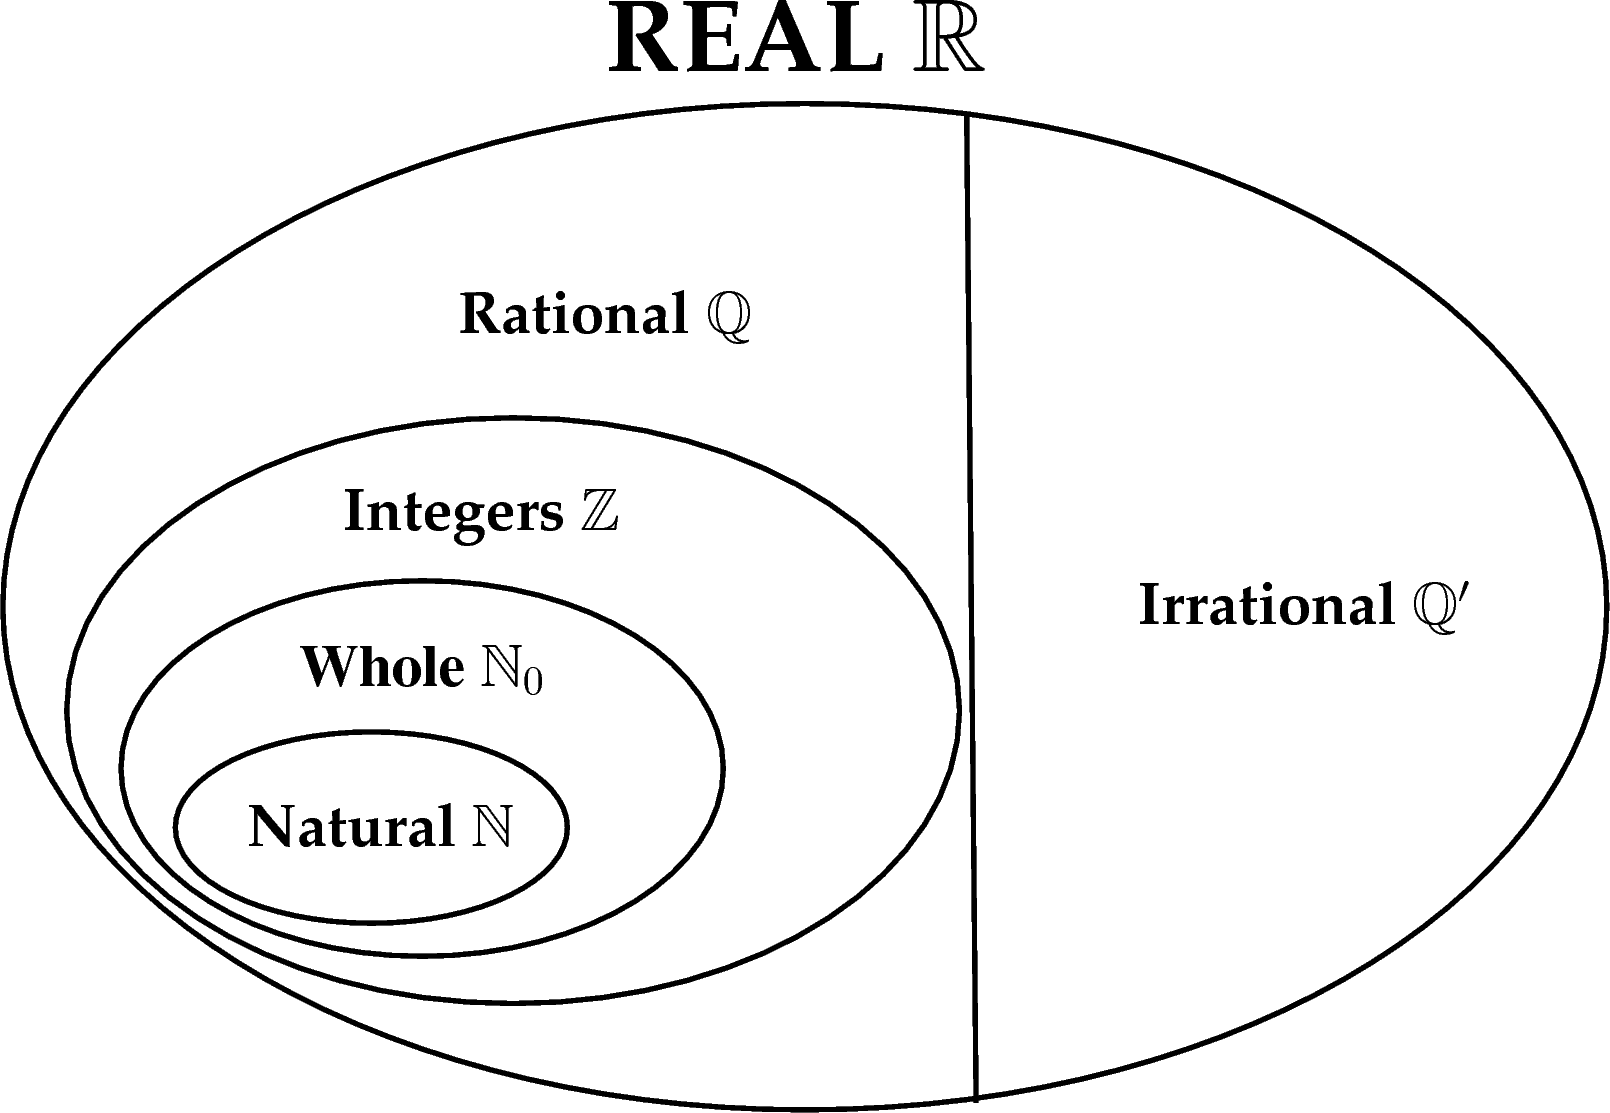
\includegraphics[width=9cm]{col11306.imgs/m38348_MG10C3_001.png} % m38348;MG10C3\_001.png;;;6.0;8.5;
\scalebox{0.6} % Change this value to rescale the drawing.
{
\begin{pspicture}(0,-4.764375)(14.481563,4.804375)
\psellipse[linewidth=0.04,dimen=outer](6.81,-0.484375)(6.81,4.28)
\psline[linewidth=0.04cm](8.18,3.695625)(8.26,-4.684375)
\psellipse[linewidth=0.04,dimen=outer](4.34,-1.364375)(3.8,2.5)
\psellipse[linewidth=0.04,dimen=outer](3.57,-1.854375)(2.57,1.61)
\usefont{T1}{ppl}{b}{n}
\rput(6.735781,4.350625){\Huge REELE $\mathbb{R}$}
\usefont{T1}{ppl}{b}{n}
\rput(11.03875,-0.484375){\Large Irrasionaal $\mathbb{Q'}$}
\usefont{T1}{ppl}{b}{n}
\rput(5.11875,1.975625){\Large Rasionaal $\mathbb{Q}$}
\usefont{T1}{ppl}{b}{n}
\rput(4.06875,0.275625){\Large Heel $\mathbb{Z}$}
\usefont{T1}{ppl}{b}{n}
\rput(3.21875,-2.324375){\Large Natuurlike $\mathbb{N}$}
\psellipse[linewidth=0.04,dimen=outer](3.14,-2.354375)(1.68,0.83)
\usefont{T1}{ptm}{b}{n}
\rput(3.5735939,-1.024375){\Large Tel $\mathbb{N}_0$}
\end{pspicture} 
}
\vspace{2pt}
\vspace{.1in}
\end{center}
\end{figure}       
\par 
Ons gebruik die volgende definisies:\par 
\begin{itemize}[itemsep=5pt]
\item natuurlike getalle is $\{1; 2; 3; \ldots\}$
\item telgetalle is $\{0; 1; 2; 3; \ldots\}$
\item heelgetalle is $\{\ldots -3; -2; -1; 0; 1; 2; 3; \ldots\}$
\end{itemize}

\nopagebreak
 $ \hspace{-5pt}\begin{array}{cccccccccccc}   \end{array} $ \hspace{2 pt}\raisebox{-0.2em}{
\includegraphics[height=1em]{../icons/www.pdf}} {(subsection shortcode: MG10036 )} \par 

\Definition{Rasionale getal}{
’n Rasionale getal is enige getal wat geskryf kan word as: 
%       \label{m38348*uid6}\nopagebreak\noindent{}

\begin{equation*}
\frac{a}{b}
\end{equation*}
waar $a$ en $b$ heelgetale is en $b\ne 0$. \par 
} 


Die volgende getalle is almal rasionaal.\par 
\nopagebreak\noindent{}

\begin{equation*}
\frac{10}{1};\frac{21}{7};\frac{-1}{-3};\frac{10}{20};\frac{-3}{6}
\end{equation*}
Jy kan sien dat al die tellers en noemers heelgetalle is.\par 

\par
Dit beteken dat alle heelgetalle rasionaal is, aangesien hulle geskryf kan word met ’n noemer van $1$.\par 
Dus is

\begin{equation*}
\frac{\sqrt{2}}{7} ; \frac{20}{\pi}
\end{equation*}
nie voorbeelde van rasionale getalle nie, want in elke geval is óf die teller óf die noemer nie ’n heelgetal nie.\par 
’n Getal wat nie geskryf word in die vorm van ’n heelgetal gedeel deur ’n heelgetal nie kan nogtans ’n rasionale
getal wees. Dit is omdat die vereenvoudigde resultaat wel as ’n kwosiënt van heelgetalle geskryf kan word. Die
reël is dat indien ’n getal geskryf kan word as ’n kwosiënt van heelgetalle, dit rasionaal is, selfs al kan dit op ’n
manier geskryf word wat nie so ’n kwosiënt is nie. Hier is twee voorbeelde wat dalk nie na rasionale getalle lyk
nie, maar nogtans is, omdat daar ekwivalente vorms gevind kan word wat bestaan uit ’n heelgetal gedeel deur ’n
heelgetal:\par 
\nopagebreak\noindent{}
\begin{equation*}    
\frac{-1,33}{-3}=\frac{133}{300}; ~~~~~~\frac{-3}{6,39}=\frac{-300}{639}=\frac{-100}{213}
\end{equation*}


\subsection*{Decimal numbers}
\addcontentsline{toc}{subsection}{Decimal numbers}
\nopagebreak
 $ \hspace{-5pt}\begin{array}{cccccccccccc}   \end{array} $ \hspace{2 pt}\raisebox{-0.2em}{
\includegraphics[height=1em]{../icons/www.pdf}} {(subsection shortcode: MG10037 )} \par 
Alle heelgetalle en heeltallige kwosiënte is rasionaal. Daar is twee bykomende vorme van rasionale getalle.\par 




\begin{activity}{Decimal numbers }
\nopagebreak
Jy kan die rasionale getal
$\frac{1}{2}$ skryf as die desimale getal $0,5$. Skryf die volgende getalle as desimale getalle:\par 
\begin{enumerate}[itemsep=5pt, label=\textbf{\arabic*}. ] 
\item $\dfrac{1}{4}$
\item $\dfrac{1}{10}$
\item $\dfrac{2}{5}$
\item $\dfrac{1}{100}$
\item $\dfrac{2}{3}$
\end{enumerate}
Beskou die getalle na die desimale komma. Kom hulle tot ’n einde of gaan hulle voort? Indien hulle voortgaan, is
daar ’n herhalende patroon in die getalle? \par 
\end{activity}

Jy kan ’n rasionale getal as ’n desimale getal skryf. Twee tipes desimale getalle wat as rasionale getalle geskryf
kan word:\par 
\begin{itemize}
\item Desimale getalle waarvan die nie-nul getalle na die komma tot ’n einde kom of termineer, byvoorbeeld die breuk
 $\dfrac{4}{10}$ kan geskryf word as $0,4$.
\item Desimale getalle wat ’n nimmereindigende herhalende patroon van getalle na die komma het, byvoorbeeld die breuk$\dfrac{1}{3}$ kan geskryf word as
$0,\dot{3}$. 
Die dot beteken dat die $3$’e repeteer, m.a.w. $0,333\ldots=0,\dot{3}$.
\end{itemize}


\Tip{Jy kan ’n kol oor die herhalende desimale aanbring om aan te dui dat die desimaal repeterend is.}

\par

\subsection*{Omskakeling tussen terminerende desimale getalle en rasionale getalle}
\addcontentsline{toc}{subsection}{Omskakeling tussen terminerende desimale getalle en rasionale getalle}
’n Desimale getal het ’n heeltallige deel en ’n breukdeel. Byvoorbeeld, $10,589$ het ’n heeltallige deel van $10$ en ’n
breukdeel van $0,589$ omdat $10+0,589=10,589$. Die breukdeel kan geskryf word as ’n rasionale getal, m.a.w.
met ’n teller en ’n noemer wat heelgetalle is. \\
\\
Elke syfer na die desimale komma is ’n breuk met ’n noemer wat ’n vermeerderende mag van $10$ is. Byvoorbeeld: 
\begin{itemize}
 \item $0,1$ is $\dfrac{1}{10}$
\item $0,01$ is $\dfrac{1}{100}$
\item $0,001$ is $\dfrac{1}{1000}$
\end{itemize}

Dit beteken dat:
\begin{equation*}
 \begin{array}{lll}10,589& = &10 + \dfrac{5}{10} + \dfrac{8}{100} + \dfrac{9}{1000} &\\ 
  &=& 10 \dfrac{589}{1000} \\
\\
&=& \dfrac{10589}{1000}
 \end{array}

\end{equation*}

\subsection*{Converting recurring decimals into rational numbers}

 $ \hspace{-5pt}\begin{array}{cccccccccccc}   \end{array} $ \hspace{2 pt}\raisebox{-0.2em}{
\includegraphics[height=1em]{../icons/www.pdf}} {(subsection shortcode: MG10039 )} \par 

Wanneer die desimaal repeterend is, is daar ’n bietjie meer werk nodig om die breukdeel van die desimale getal
as ’n breuk te skryf.\par 

\begin{wex}
{%title
Converting decimal numbers to fractions
}
{%question
\\
Indien ons $0,\dot{3}$ in die vorm $\dfrac{a}{b}$ wil skryf(waar $a$ en $b$ heelgetalle is)
}
{%answer

\westep{Define an equation}
Let $x = 0,33333\ldots$


\westep{vermenigvuldig met $10$ aan beide kante}

$10x = 3,33333\ldots$


\westep{trek die tweede verg. van die eerste verg. af}

$9x = 3 $

\westep{Simplify}

$ x = \dfrac{3}{9} = \dfrac{1}{3} $
}
\end{wex}


\begin{wex}
{%title
Converting decimal numbers to fractions
}
{%question
\\skryf $5,\dot{4}\dot{3}\dot{2}$ as 'n rasionale breuk
}
{%answer

\westep{Define an equation}

$$ x = 5,432432432\ldots $$

\westep{vermenigvuldig met $1000$ aan beide kante}

$$ 1000x = 5432,432432432\ldots $$

\westep{trek die tweede verg. van die eerste verg. af}

$$ 999x = 5427 $$

\westep{Vireenvodig}

$$ x = \dfrac{5427}{999} = \dfrac{201}{37} $$

}
\end{wex}




In die eerste voorbeeld is die desimaal vermenigvuldig met $10$  en in die tweede voorbeeld is dit vermenigvuldig met $1000$. Dit is omdat daar in die eerste voorbeeld slegs een repeterende syfer (nl. $3$) was, terwyl die tweede voorbeeld drie repeterende syfers (i.e. $432$) gehad het.\par 
In die algemeen, as jy een repeterende syfer het, vermenigvuldig jy met $10$.  As jy twee repeterende syfers het,
vermenigvuldig jy met $100$.  Met drie syfers vermenigvuldig jy met $1000$ en so aan.\par

Nie alle desimale getalle kan as rasionale getalle geskryf word nie. Hoekom nie? Irrasionale desimale getalle soos
$\sqrt{2}=1,4142135\ldots$
kan nie geskryf word met ’n heeltallige teller en noemer nie, omdat daar geen patroon van repeterende syfers is nie. Jy behoort egter, so ver moontlik, eerder rasionale getalle of breuke as desimale getalle te gebruik.

% \label{m38348*secfhsst!!!underscore!!!id606}




\section{Irrational numbers}
\setcounter{figure}{1}
\setcounter{subfigure}{1}


 $ \hspace{-5pt}\begin{array}{cccccccccccc}   \end{array} $ \hspace{2 pt}\raisebox{-0.2em}{
\includegraphics[height=1em]{../icons/www.pdf}} {(subsection shortcode: MG10055 )} \par 
Jy het reeds gesien dat baie ink en papier nodig sou wees om repeterende desimale getalle neer te skryf. Dis
nie net onmoontlik om hierdie getalle neer te skryf nie, maar om énige getal tot baie desimale plekke of met hoë
akkuraatheid neer te skryf, is gewoonlik onprakties. Daarom benader ons dikwels ’n getal tot ’n sekere aantal
desimale plekke of, selfs beter, tot ’n sekere aantal beduidende syfers.\par 

\Definition{Irrational numbers}{Irrasionale getalle is getalle wat nie as ’n breuk met ’n heeltallige teller en noemer geskryf kan word nie. Dit
beteken dat enige getal wat nóg ’n eindige nóg ’n herhalende desimale getal is, irrasionaal is. 
}

Voorbeelde van irrasionale getalle is:\par 

\begin{equation*}
\sqrt{2};~\sqrt{3};~\sqrt[3]{4};~\pi ;
~\frac{1+\sqrt{5}}{2}\approx 1,618
\end{equation*}




\Tip{Wanneer irrasionale getalle in desimaalnotasie geskryf word, het hulle ’n oneindige aantal desimale syfers wat nooit herhaal nie. \\The square roots of non-perfect squares and the cube roots of non-perfect cubes are all irrational.}

As jy gevra word om uit te werk of ’n getal rasionaal of irrasionaal is, skryf eers die getal in desimaalnotasie. As die desimaal eindig, is die getal rasionaal. As dit vir ewig aanhou, soek vir ’n herhalende syferpatroon. As daar geen patroon is nie, is die getal irrasionaal.\par 
As jy ’n irrasionale getal in desimaalnotasie skryf, kan jy (as jy baie tyd en papier het!) aanhou skryf vir baie, baie
syfers. Dit is egter ongeriefliek en ’n mens rond gewoonlik af.\par 



\begin{activity}{Irrational numbers }
\nopagebreak
Watter van die volgende kan nie as 'n rasionale getalle geskryf word nie?\par \vspace{0.5cm}
\textbf{Remember}: ’n Rasionale getal is ’n breuk met ’n heeltallige teller en noemer. Eindige en herhalende desimale
getalle is rasionaal.\par 
\begin{enumerate}[itemsep=5pt, label=\textbf{\arabic*}. ] 
\item $\pi =3,14159265358979323846264338327950288419716939937510\ldots$
\item $1,4$
\item $1,618\phantom{\rule{0.166667em}{0ex}}033\phantom{\rule{0.166667em}{0ex}}989\phantom{\rule{0.166667em}{0ex}}\ldots$
\item $100$
\item $1,7373737373\ldots$
\item $0,\overline{02}$
\end{enumerate}
\end{activity}


\begin{exercises}{}{
\begin{enumerate}[itemsep=5pt, label=\textbf{\arabic*}. ] 
\item As $a$ 'n heel getal is, $b$ 'n heel getal is en $c$ is irrasionaal, watter van die volgende is rasionale getalle? 
  \begin{enumerate}[itemsep=5pt, label=\textbf{\alph*}. ] 
    \item $\dfrac{5}{6}$
    \item $\dfrac{a}{3}$
    \item $\dfrac{-2}{b}$
    \item $\dfrac{1}{c}$
    \end{enumerate}
\item As $\dfrac{a}{1}$ 'n rasionale getal is, watter van die volgende is valid values for $a$?
    \begin{enumerate}[itemsep=5pt, label=\textbf{\alph*}. ] 
    \item $1$
    \item $-10$
    \item $\sqrt{2}$
    \item $2,1$
    \end{enumerate}
%         \end{enumerate}
% \par \raisebox{-0.2em}{
\includegraphics[height=1em]{../icons/www.pdf}} Find the answers with the shortcodes:
%  \par \begin{tabular}[h]{cccccc}
%  (1.) l35  &  (2.) l3N  & \end{tabular}}
% \end{exercises}
% 
%            \begin{exercises}{Fractions }{
%             \nopagebreak
%       \label{m38348*id63882}\begin{enumerate}[itemsep=5pt, label=\textbf{\arabic*}. ] 
\item Skryf die volgende as breuke:
    \begin{enumerate}[itemsep=5pt, label=\textbf{\alph*}. ] 
    \item $0,1$
    \item $0,12$
    \item $0,58$
    \item $0,2589$
    \end{enumerate}
%         \end{enumerate}
% \par \raisebox{-0.2em}{
\includegraphics[height=1em]{../icons/www.pdf}} Find the answers with the shortcodes:
%  \par \begin{tabular}[h]{cccccc}
%  (1.) l3R  & \end{tabular}}
% \end{exercises}
% 
% \begin{exercises}{Repeated Decimal Notation }{
% %             \nopagebreak
%       \label{m38348*id64513}\begin{enumerate}[itemsep=5pt, label=\textbf{\arabic*}. ] 
\item Skryf die volgende in repeterende(herhalende) desimale notasie:
    \begin{enumerate}[itemsep=5pt, label=\textbf{\alph*}. ] 
    \item $0,11111111\ldots$
    \item $0,1212121212\ldots$
    \item $0,123123123123\ldots$
    \item $0,11414541454145\ldots$
    \end{enumerate}
\item Skryf die volgende in repeterende(herhalende) desimale notasie:
    \begin{enumerate}[itemsep=5pt, label=\textbf{\alph*}. ] 
    \item $\dfrac{2}{3}$
    \item $1\dfrac{3}{11}$
    \item $4\dfrac{5}{6}$
    \item $2\dfrac{1}{9}$
    \end{enumerate}
\item Skryf die volgende in breukvorm:
    \begin{enumerate}[itemsep=5pt, label=\textbf{\alph*}. ] 
    \item $0,\dot{5}$
    \item $0,6\dot{3}$
    \item $5,\overline{31}$
    \end{enumerate}
\end{enumerate}
% \par \raisebox{-0.2em}{
\includegraphics[height=1em]{../icons/www.pdf}} Find the answers with the shortcodes:
%  \par \begin{tabular}[h]{cccccc}
%  (1.) l3U  &  (2.) l3n  &  (3.) l3Q  & \end{tabular}}
\end{exercises}

\section{ Afronding}
\nopagebreak
$ \hspace{-5pt}\begin{array}{cccccccccccc}   
\includegraphics[width=0.75cm]{col11306.imgs/summary_fullmarks.png} &   \end{array} $ \hspace{2 pt}\raisebox{-5 pt}{} {(section shortcode: MG10057 )} \par 
Afronding van ’n desimale getal tot ’n sekere aantal desimale plekke is ’n eenvoudige manier om die benaderde
waarde van ’n desimale getal te vind. As jy byvoorbeeld $2,6525272$ wil afrond tot drie desimale plekke, tel jy drie
plekke na die desimale komma af en plaas ’n $|$ tussen die derde en die vierde syfer na die desimale komma.\par 

\begin{equation*}
2,652|5272
\end{equation*}
Nadat jy vasgestel het of die syfer in die derde desimale plek na bo of na onder afgerond moet word, word al
die syfers aan die regterkant van die $|$ geïgnoreer. Jy rond die finale syfer na bo af as die eerste syfer ná die $|$ groter of gelyk is aan $5$ andersins rond jy na onder af (los die syfer onveranderd). Wanneer die eerste syfer links
van die $|$ 'n $9$ is en jy moet boontoe afrond, dan word die $9$ 'n $0$ en die tweede syfer links van die  $|$ word boontoe afgerond.\par 
Dus, aangesien die eerste syfer na die $|$ 'n 5 is, moet ons afrond na bo en die derde desimaal na die komma word 3 Die antwoord vir $2,6525272$ afgerond na drie desimale pleke is dus $2,653$.
\par


\begin{wex}{Afronding }

{ Rond die volgende getalle af: 
\begin{enumerate}[itemsep=5pt, label=\textbf{\arabic*}. ] 

\item $\frac{120}{99}=1,212121212\dot{1}\dot{2}$ tot $3$ desimale plekke
\item $\pi =3,141592654\ldots$ tot $4$ desimale plekke
\item $\sqrt{3}=1,7320508\ldots$ tot $4$ desimale plekke
\item $2,78974526\ldots$ tot $3$ desimale plekke
\end{enumerate}
}
{

\westep{Mark off the required number of decimal places}

\begin{enumerate}[itemsep=5pt, label=\textbf{\arabic*}. ] 
\item $\frac{120}{99}=1,212|121212\dot{1}\dot{2}$
\item $\pi =3,1415|92654\ldots$
\item $\sqrt{3}=1,7320|508\ldots$
\item $2,789|74526\ldots$
\end{enumerate}

\westep{Check next digit to see if you must round up or round down}
\begin{enumerate}[itemsep=5pt, label=\textbf{\arabic*}. ]
\item Die laast syfer van $\frac{120}{99}=1,212|121212\dot{1}\dot{2}$  moet na onder afgerond word.
\item Die laast syfer van $\pi =3,1415|92654\ldots$ moet na bo afgerond word.
\item Die laast syfer van $\sqrt{3}=1,7320|508\ldots$ moet na bo afgerond word.
\item Die laast syfer van $2,789|74526\ldots$ moet na bo afgerond word.  
\newline Aangesien dit ’n $9$, is, vervang ons dit met $0$ en
rond die tweede laaste syfer boontoe af.
\end{enumerate}

\westep{Write final answer}
\begin{enumerate}[itemsep=5pt, label=\textbf{\arabic*}. ]
\item $\frac{120}{99}=1,212$ afgerond tot $3$ desimale plekke
\item $\pi =3,1416$  afgerond tot $4$ desimale plekke
\item $\sqrt{3}=1,7321$ afgerond tot $4$ desimale plekke
\item $2,790$
\end{enumerate}
}  
\end{wex}

}

\begin{exercises}{}
{
Gebruik jou sakrekenaar om die volgende irrasionale getalle tot $3$ desimale plekke te skryf:
\begin{enumerate}[itemsep=5pt, label=\textbf{\arabic*}. ]
 \item $4\pi$
\item $\sqrt{11}$
\item $\dfrac{0,8}{3}$
\item $\sqrt[3]{7}$
\item $2\sqrt{10}$
\item $\dfrac{1}{18}$
\end{enumerate}

}
\end{exercises}


\section{Estimating surds}
\setcounter{figure}{1}
\setcounter{subfigure}{1}
 $ \hspace{-5pt}\begin{array}{cccccccccccc}   
\includegraphics[width=0.75cm]{col11306.imgs/summary_fullmarks.png} &   \end{array} $ \hspace{2 pt}\raisebox{-5 pt}{} {(subsection shortcode: MG10052 )} \par 
Indien die ${n}^{\mathrm{th}}$ magswortel van ’n getal nie as ’n rasionale getal geskryf kan word nie,  noem ons dit ’n wortelgetal . Byvoorbeeld, $\sqrt{2}$ en $\sqrt[3]{6}$ is wortelgetalle, maar $\sqrt{4}$ is nie ’n wortelgetal nie, aangesien ons dit kan vereenvoudig tot die rasionale getal $2$.\par 
In hierdie hoofstuk gaan ons slegs wortelgetalle van die vorm $\sqrt[n]{a}$, ondersoek, waar  $a$ ’n positiewe heelgetal is, byvoorbeeld $\sqrt{7}$ or $\sqrt[3]{5}$. Dit is algemeen dat $n$ to be $2$, daarom skryf ons $\sqrt[2]{a}$. in plaas van $\sqrt{a}$.\par 
Dit is soms nuttig om ’n wortelgetal te benader sonder om ’n sakrekenaar te gebruik. Ons wil, byvoorbeeld, kan benader waar $\sqrt{3}$ op die getallelyn lê. Met ’n sakrekenaar kan ons bereken $\sqrt{3}$ is gelyk aan $1,73205\ldots$. Dit is maaklik on te sien dat $\sqrt{3}$ bo $1$ en onder $2$ lê. Om sonder ’n sakrekenaar te bepaal waar ander wortelgetalle, soos $\sqrt{18}$ op die getallelyn lê, moet jy eers die volgende verstaan:\par 


\Identity{}{
\begin{center}
As $a$ en $b$ positiewe getalle is met $a\lessthan{}b$, dan $\sqrt[n]{a}\lessthan{}\sqrt[n]{b}$. 
\end{center}}
\par
       
\Note{’n Volkome vierkant is die getal wat verkry word wanneer ’n heelgetal met homself vermenigvuldig word. Byvoorbeeld, $9$  is ’n volkome vierkant aangesien ${3}^{2}=9$. \\Soortgelyk is ’n volkome derdemag die getal wat verkry word wanneer ’n heelgetal
tot die derde mag verhef word. Byvoorbeeld, $27$ is ’n volkome derdemag aangesien ${3}^{3}=27$.}



Gegee die wortelgetal $\sqrt[3]{52}$, behoort jy te kan sien dat dit iewers tussen $3$ en $4$,lê op die getallelyn, aangesien $\sqrt[3]{27}=3$ en $\sqrt[3]{64}=4$ en $52$ tussen $27$ en $64$.Jou sakrekenaar sal dit bevestig: $\sqrt[3]{52}=3,73\ldots$ which is indeed between $3$ and $4$.\par 

\begin{wex}{Estimating surds}
{
Vind die opeenvolgende heelgetalle wat weerskante van $\sqrt{26}$ lê.
(Onthou dat opeenvolgende heelgetalle met $1$ verskil. byvoorbeeld $5$ en $6$ of $8$ en $9$).
}
{
           
\westep{Gebruik die volkome vierkant om die laer heel getal te raai}     
${5}^{2}=25$. Daarom $5\lessthan{}\sqrt{26}$.

\westep{gebruik die volkome vierkant on die hoer heel getal te raai}
${6}^{2}=36$. 
Daarom $\sqrt{26}\lessthan{}6$.

\westep{Die finale aantwoord is}
$5\lessthan{}\sqrt{26}\lessthan{}6$. 
}
\end{wex}


\begin{wex}{Benadering van wortelgetalle }{

Vind die opeenvolgende heelgetalle wat weerskante van $\sqrt[3]{49}$ lê.
}
{
\westep{Gebruik volkome derdemagte om die laer heel getal te raai}   ${3}^{3}=27$, daarom $3\lessthan{}\sqrt[3]{49}$.

\westep{Gebruik volkome derdemagte om die hoer heel getal te raai} ${4}^{3}=64$, daarom $\sqrt[3]{49}\lessthan{}4$. 

\westep{Die antwoord is}
$3\lessthan{}\sqrt[3]{49}\lessthan{}4$

\westep{Check the answer by cubing all terms in the inequality and then simplify}
$27<49<64$. wat waar is, dus lê $\sqrt[3]{49}$ tussen $3$ en $4$.
%       \end{enumerate}
}
\end{wex}

\begin{exercises}{}
 {
Vind twee opeenvolgende heelgetalle wat weerskante van die getalle lê, sonder die gebruik van a sakrekenaar:
\begin{enumerate}[itemsep=5pt, label=\textbf{\arabic*}. ]
\item $\sqrt{18}$
\item $\sqrt{29}$
\item $\sqrt[3]{5}$
\item $\sqrt[3]{79}$

\end{enumerate}

\end{exercises}



\section{Products}
\setcounter{figure}{1}
\setcounter{subfigure}{1}
 $ \hspace{-5pt}\begin{array}{cccccccccccc}   
\includegraphics[width=0.75cm]{col11306.imgs/summary_fullmarks.png} &   \end{array} $ \hspace{2 pt}\raisebox{-5 pt}{} {(section shortcode: MG10060 )} \par 
%   
\nopagebreak
Wiskundige uitdrukkings is soos sinne en elke deel het ’n spesifieke naam. Jy behoort vertroud te wees met die
volgende name wat die dele van wiskundige uitdrukkings beskryf.\par 

\begin{equation*}
3x^2 + 7xy -14 = 0
\end{equation*}



\begin{table}[H]
\begin{center}
\begin{tabular}{|l|l|}
\hline
\textbf{Name} & \textbf{Examples} \\
\hline
terms & $3x^2;~ 7xy;~ -14$\\ \hline
expression & $3x^2 + 7xy -14$\\ \hline
coefficient & $3;~7$\\ \hline
exponent & $2;~1$\\ \hline
base & $x;~y$\\ \hline
constant & $3;~7;-14$\\ \hline
variable & $x;~ y$\\ \hline
equation & $3x^2 + 7xy -14 = 0$\\ \hline
binomial & expression with two terms\\ \hline
trinomial & expression with three terms \\ \hline

% \label{m39387*secfhsst!!!underscore!!!id1562}\vspace{.5cm}

\end{tabular}
\end{center}
\end{table} 

\par

\subsection*{Multiplying a monomial and a binomial}

\begin{wex}{Applying the distributive law}
{Write the following without brackets in its simplest form: $2a(a-1) - 3(a^{2}-1)$}
{
\westep{Toepassing van die distributiewe wet}
\begin{equation*}
\begin{array}{lll} 2a(a-1) -3(a^{2}-1) &=& 2a(a) + 2a(-1) + (-3)(a^{2})+(-3)(-1) &
&=& 2a^{2} - 2a - 3a^{2} + 3
\end{array}
\end{equation*}

\westep{Simplify}
\begin{equation*}
\begin{array}{lll} &=& -a^{2} -2a + 3 & 
\end{array}
\end{equation*}
}
\end{wex}

\subsection*{Produk van twee Binomiale}
\addcontentsline{toc}{subsection}{Multiplying two binomials}

’n Binomiaal is ’n wiskundige uitdrukking met twee terme, soos $ax+b$ and $cx+d$. As hierdie twee binomiale
vermenigvuldig word, is die volgende die resultaat:
\begin{equation*}
\begin{array}{ccc}\hfill (ax+b)(cx+d) & =& (ax)(cx)+(ax)d+b(cx)+bd\hfill  \\
& =& ac{x}^{2}+adx +bcx+bd\hfill\\
& =& ac{x}^{2}+x(ad+bc)+bd\hfill \end{array}
\end{equation*}

\Note{You may use FOIL = F(firsts) O(outers) I(inners) L(lasts) to remember this technique}
\par

\begin{wex}{Produk van twee binomiale }
{Find the product of $(3x-2)$ and $(5x+8)$ }{
\westep{vind die produk van}
\begin{equation*}
\begin{array}{ccl}\hfill (3x-2)(5x+8)& =& (3x)(5x)+(3x)(8)+(-2)(5x)+(-2)(8)\hfill \\
 & =& 15{x}^{2}+24x-10x-16\hfill \\
 & =& 15{x}^{2}+14x-16\hfill 
\end{array}
\end{equation*}
} 
\end{wex}




Die produk van twee identiese binomiale, is bekend as die kwadraat (of vierkant) van binomiale en word geskryf
as:

\begin{equation*}
{(ax+b)}^{2}={a}^{2}{x}^{2}+2abx+{b}^{2}
\end{equation*}
Gestel die twee terme is $ax+b$, en $ax-b$ dan is hulle produk:\par 

\begin{align*}
(ax+b)(ax-b) &={a}^{2}{x}^{2}-{b}^{2} \\ &= (ax)^2-b^2
\end{align*}

Dit staan bekend as die verskil van twee kwadrate (of vierkante).\par 


\subsection*{ Multiplying a binomial and a trinomial}
\addcontentsline{toc}{subsection}{Multiplying a binomial and a trinomial}

\setcounter{subfigure}{0}


\begin{figure}[H] % horizontal\label{m39387*productpolynomials}


\textnormal{Khan Academy video on products of polynomials.}\vspace{.1in} \nopagebreak
\label{m39387*yt-media1}\label{m39387*yt-video1}
\raisebox{-5 pt}{ 
\includegraphics[width=0.5cm]{col11306.imgs/summary_www.png}} { (Video:  MG10062 )}

\end{figure}   

\addtocounter{footnote}{-0}

n trinomiaal of drieterm is 'n uitdrukking met drie terme, byvoorbeeld $ax^{2} + bx + c$.
In hierdie gedeelte, gaan ons leer hoe om ’n binomiaal met ’n trinomiaal of drieterm te vermenigvuldig.\par 

\Tip{In die vermenigvuldiging van die binomiaal \begin{math}A+B\end{math} met die trinomiaal \begin{math}C+D+E\end{math}, is die heel eerste stap om die distributiewe wet toe te pas:


 $(A+B)(C+D+E)= A(C+D+E)+B(C+D+E) $

}

As jy dit onthou, sal jy nie ’n fout maak nie!}

\begin{wex}
{Vermenigvuldiging van Binomiaal met Trinomiaal 
}
{
Vermenigvuldig$x-1$ met ${x}^{2}-2x+1$.
} 
{
\westep{Pas die distributiewe wet toe}
$
(x-1)(x^2-2x+1) &= x(x^2-2x+1)-1(x^2-2x+1)
$

\westep{brei die hakies uit}

$
\phantom{(x-1)(x^2-2x+1) } = x^3-2x^2+x-x^2+2x-1
$

\westep{vereenvoudig}

$
\phantom{(x-1)(x^2-2x+1) } = x^3-3x^2 + 3x1
$


}       

\end{wex}



\begin{exercises}{}
Vind die produk van:

\begin{multicols}{2}
\begin{enumerate}[label=\textbf{\arabic*}., itemsep=5pt]
\item $2y(y+4)$ 
\item $(y+5)(y+2) $
\item $(2-t)(1-2t)$
\item $(x-4)(x+4)$
\item $ (2p+9)(3p+1)$
\item $(3k-2)(k+6)$
\item $(s+6)^2$
\item $-(7-x)(7+x)$
\item $(3x-1)(3x+1)$
\item $(7k+2)(3-2k)$
\item $(1-4x)^2$
\item $(-3-y)(5-y)$
\item $(8-x)(8+x)$
\item $(9+x)^2$
\item$(-2{y}^{2}-4y+11)(5y-12)$ 
\item$(7{y}^{2}-6y-8)(-2y+2)$% make-rowspan-placeholders
\item$(10{y}^{5}+3)(-2{y}^{2}-11y+2)$ 
\item$(-12y-3)(12{y}^{2}-11y+3)$% make-rowspan-placeholders
\item$(-10)(2{y}^{2}+8y+3)$ 
\item$(2{y}^{6}+3{y}^{5})(-5y-12)$% make-rowspan-placeholders
\item$(-7y+11)(-12y+3)$% make-rowspan-placeholders
\item$(7y+3)(7{y}^{2}+3y+10)$% make-rowspan-placeholders
\item$(9)(8{y}^{2}-2y+3)$ 
\item$(-6{y}^{4}+11{y}^{2}+3y)(10y+4)(4y-4)$ 
\end{enumerate}
\end{multicols}
\end{exercises}





\section{Factorisation}

 $ \hspace{-5pt}\begin{array}{cccccccccccc}   
\includegraphics[width=0.75cm]{col11306.imgs/summary_fullmarks.png} &   
\includegraphics[width=0.75cm]{col11306.imgs/summary_video.png} &   \end{array} $ \hspace{2 pt}\raisebox{-5 pt}{} {(section shortcode: MG10063 )} \par 
%            \subsubsubsection{ Factorisation}
%             \nopagebreak
Faktorisering is die omgekeerde proses van die uitbreiding van hakies. Byvoorbeeld, as hakies uitgebrei word,
word $2(x+1)$ geskryf as $2x+2$. Faktorisering sal dus begin met $2x+2$ en eindig met $2(x+1)$. 

\Identity{}
{
\begin{center}
\begin{small}\hspace{8pt}expanding\end{small}\\
\begin{Large}
$2(x+1)$ \begin{Huge} $\leftrightharpoons$ \end{Huge} $2x+2$
\end{Large}\\
\begin{small}\hspace{8pt}factorising\end{small}
\end{center}
}

The two expressions $2(x+1)$ and $2x+2$ are equivalent; they have the same value for all values of $x$



\par
In vorige grade het ons gefaktoriseer deur die uithaal van gemeenskaplike faktore en die verskil tussen twee vierkante.\par 

\subsection*{Common factors}
\nopagebreak
Faktorisering deur die uithaal van gemeenskaplike faktore, is gebaseer daarop dat daar faktore is wat in al die terme voorkom. \par

Byvoorbeeld, $2x-6{x}^{2}$ kan as volg gefaktoriseer word:\par 

\begin{equation*}
2x-6{x}^{2}=2x(1-3x)
\end{equation*}

\Tip{Check your answer by multiplying the bracket out and make sure you get back to the original expression. 
\begin{equation*}
 2x(1-3x) = 2x - 6x^{2}
\end{equation*}
is correct.
}


\begin{wex}{Faktorisering}
{Factorise completely: ${b}^{2}{y}^{5}-3ab{y}^{3}$}
{
\westep{Take out the highest common factor $by^3$}  
\begin{equation*}
{b}^{2}{y}^{5}-3ab{y}^{3}& =& b{y}^{3}(b{y}^{2}-3a)
\end{equation*}
}
\end{wex}

\begin{wex}{ Faktorisering wat die omruiling van getalle in hakies benodig: }{Faktoriseer: $5(a-2)-b(2-a)$ }{
\westep{In this case use a ``switch around'' strategy to find the common factor. Notice that $2-a = -(a-2)$ }
\begin{equation*}
\begin{array}{ccl}
\hfill 5(a-2)-b(2-a)& =& \hfill 5(a-2)-[-b(a-2)]  \\
&= & 5(a-2)+b(a-2)\\ 
& =& (a-2)(5+b) \hfill
\end{array}
\end{equation*}
}
\end{wex}

\begin{exercises}{}

Vind die grootste gemene faktore van die volgende pare terme:\par

\begin{multicols}{2}
\begin{enumerate}[label=\textbf{\arabic*}., itemsep=5pt]
\item $6y;~18x$
\item $12mn;~8n$
\item $3st;~4su$ 
\item $18kl;~9kp$
\item $abc;~ac$% 
\item $2xy;~4xyz$
\item $3uv;~6u$ 
\item $9xy;~15xz$
\item $24xyz;~16yz$
\item $3m;~45n$
\end{enumerate}
\end{multicols}

\end{exercises}

\subsection* {Verskil van twee kwadrate}
Ons het gesien dat: 
\begin{equation*}
(ax+b)(ax-b)~\mbox{ Kan uit gebrui word as }~{a}^{2}{x}^{2}-{b}^{2}
\end{equation*}

Dus
\begin{equation*}
{a}^{2}{x}^{2}-{b}^{2}~\mbox{ gefaktoriseer kan word as: }~(ax+b)(ax-b)
\end{equation*}
Byvoorbeeld, ${x}^{2}-16$ kan geskryf word as $({x}^{2}-{4}^{2})$ wat die verskil is tussen twee kwadrate. 
\\Dus, die faktore van ${x}^{2}-16$ is $(x-4)$ en $(x+4)$.\par 


\Tip{When factorising look for expressions
\begin{itemize}
\item consisting of two terms 
\item with terms that have different signs (one positive, one negative)
\item with each term a perfect square 
\end{itemize}
For example $a^{2}-1;~ 4x^{2}-y^{2};~ -49+p^{4}$
}



\begin{wex}{}
{Faktoriseer volledig $3a(a^2-4)-7(a^2-4)$ \par }

{
\westep{haal die gemene faktor uit $(a^2-4)$}


\begin{equation*}
\begin{array}{ccc}\hfill 3a(a^2-4)-7(a^2-4)& =& (a^2-4)(3a-7)\hfill \end{array}
\end{equation*}

\westep{Faktoriseer die verskil is tussen twee kwadrate. $(a^2-4)$ }

$$
(a^2-4)(3a-7) = (a-2)(a+2)(3a-7)
$$

}
\end{wex}


\begin{exercises}{}{
Faktoriseer:
\begin{multicols}{2}
\begin{enumerate}[itemsep=5pt, label=\textbf{\arabic*}. ] 
\item $2l+2w$
\item $12x+32y$
\item $6{x}^{2}+2x+10{x}^{3}$
\item $2x{y}^{2}+x{y}^{2}z+3xy$
\item $-2a{b}^{2}-4{a}^{2}b$
\item $7a+4$ 
\item $20a-10$ 
\item $18ab-3bc$
\item $12kj+18kq$ 
\item $16{k}^{2}-4$ 
\item $3{a}^{2}+6a-18$
\item $-12a+24a^3$ 
\item $-2ab-8a$ 
\item $24kj-16{k}^{2}j$
\item $-{a}^{2}b-{b}^{2}a$ 
\item $12{k}^{2}j+24{k}^{2}{j}^{2}$ 
\item $72{b}^{2}q-18{b}^{3}{q}^{2}$
\item $4(y-3)+k(3-y)$ 
\item $a^2(a-1)-25(a-1)$ 
\item $bm(b+4)-6m(b+4)$
\item ${a}^{2}(a+7)+9(a+7)$ 
\item $3b(b-4)-7(4-b)$ 
\item ${a}^{2}{b}^{2}{c}^{2}-1$
\end{enumerate}
\end{multicols}
\end{exercises}



\subsection* {Factorising a quadratic trinomial }

\setcounter{subfigure}{0}
\begin{figure}[H] % horizontal\label{m39394*factorisingquadratic}
\textnormal{Khan Academy video on factorising a quadratic.}\vspace{.1in} \nopagebreak
\label{m39394*yt-media2}\label{m39394*yt-video2}
\raisebox{-5 pt}{ 
\includegraphics[width=0.5cm]{col11306.imgs/summary_www.png}} { (Video:  MG10064 )}
\vspace{2pt}
\vspace{.1in}
\end{figure}       
Faktorisering kan gesien word as die omgekeerde proses van die berekening van die produk van faktore. Om
’n kwadratiese uitdrukking te faktoriseer, is dit dus nodig om die faktore te vind wat, wanneer hulle met mekaar
vermenigvuldig word, gelyk sal wees aan die oorspronklike kwadratiese uitdrukking.\par 

Beskou ’n kwadratiese uitdrukking van die vorm: $a{x}^{2}+bx$. Ons kan sien hier is  $x$ is ’n gemeenskaplike faktor in
beide terme. Dus,$a{x}^{2}+bx$  faktoriseer tot $x(ax+b)$. Byvoorbeeld, $8{y}^{2}+4y$ faktoriseer tot  $4y(2y+1)$.\par 
’n Ander tipe kwadratiese uitdrukking bestaan uit die verskil tussen kwadrate. Ons weet dat:
\begin{equation*}
(a+b)(a-b)={a}^{2}-{b}^{2}
\end{equation*}
\\ 
So $a^2-b^2$ can be written in factorised form as $(a+b)(a-b)$ \par


Dit beteken dat wanneer ons enige kwadratiese uitdrukking wat bestaan uit die verskil tussen twee kwadrate teëkom, ons onmiddellik die faktore kan neerskryf.


Hierdie soort kwadratiese uitdrukking is eenvoudig om te faktoriseer. Nie baie kwadratiese uitdrukkings val egter
in hierdie kategorie nie, en gevolglik het ons ’n meer algemene metode nodig vir kwadrate
\par 
Ons kan leer hoe om kwadrate te faktoriseer deur twee binomiale met mekaar te vermenigvuldig en so ’n kwadratiese uitdrukking te kry. Byvoorbeeld

\begin{equation*}
\begin{array}{ccl}\hfill (x+2)(x+3)& =& x^2+3x+2x+6 \\ & =& {x}^{2}+5x+6.\hfill \end{array}
\end{equation*}
Ons kan sien dat die ${x}^{2}$ term in die kwadratiese uitdrukking die produk is van die $x$ -terme in elke hakie. Soortge-
lyk, die $6$ in die kwadratiese uitdrukking is die produk van $2$ en $3$ in die hakies. Gevolglik is die middelterm die
som van die twee terme.\par 
Dus, hoe gebruik ons hierdie inligting om die kwadratiese uitdrukking te faktoriseer?\par 
Kom ons begin faktoriseer ${x}^{2}+5x+6$ en sien of ons kan besluit op sekere algemene reëls. Eerstens, skryf twee hakies neer met ’n $x$ in elke hakie en los spasie vir die oorblywende terme.\par 
\begin{equation*}
(x\phantom{\rule{2.em}{0ex}})(x\phantom{\rule{2.em}{0ex}})
\end{equation*}
Besluit nou op die faktore van $6$.Aangesien $6$ ’n positiewe getal is, sal dit wees:\par 
% \textbf{m39394*id275986}\par
\begin{table}[H]
% \begin{table}[H]
% \\ '' '0'
\begin{center}
\label{m39394*id275986}
\noindent

\begin{tabular}[t]{|c|c|}\hline
% My position: 0
% my spanname: 
% my ct of spanspec: 0
% my column-count: 2
\multicolumn{2}{|c|}{Factors of $6$}
\\ \hline
%--------------------------------------------------------------------
$1$ &
$6$% make-rowspan-placeholders
\\ \hline
%--------------------------------------------------------------------
$2$ &
$3$% make-rowspan-placeholders
\\ \hline
%--------------------------------------------------------------------
$-1$ &
$-6$% make-rowspan-placeholders
\\ \hline
%--------------------------------------------------------------------
$-2$ &
$-3$% make-rowspan-placeholders
\\ \hline
%--------------------------------------------------------------------
\end{tabular}
\end{center}
%     \begin{center}{\small\bfseries Table 8.6}\end{center}
%     \begin{caption}{Factors of 6}\end{caption}
\end{table}
\par
\label{m39394*id276096}Vervolgens het ons nou vier moontlikhede:\par 
% \textbf{m39394*id276099}\par
\begin{table}[H]
% \begin{table}[H]
% \\ '' '0'
\begin{center}
\label{m39394*id276099}
\noindent

\begin{tabular}{|l|l|l|l|}\hline
Option 1 &
Option 2 &
Option 3 &
Option 4% make-rowspan-placeholders
\\ \hline
%--------------------------------------------------------------------
  $(x+1)(x+6)$
  &
  $(x-1)(x-6)$
  &
  $(x+2)(x+3)$
  &
  $(x-2)(x-3)$
% make-rowspan-placeholders
\\ \hline
%--------------------------------------------------------------------
\end{tabular}
\end{center}
%     \begin{center}{\small\bfseries Table 8.7}\end{center}
%     \begin{caption}{Factor Options}\end{caption}
\end{table}
\par
Vervolgens vermenigvuldig ons elke stel hakies uit om te sien watter stel gee vir die regte middelterm.\par 
% \textbf{m39394*id276265}\par
\begin{table}[H]
% \begin{table}[H]
% \\ '' '0'
\begin{center}
\label{m39394*id276265}
\noindent

\begin{tabular}[t]{|l|l|l|l|}\hline
Opsie 1 &
Opsie 2 &
Opsie 3 &
Opsie 4% make-rowspan-placeholders
\\ \hline
%--------------------------------------------------------------------
  $(x+1)(x+6)$
  &
  $(x-1)(x-6)$
  &
  $(x+2)(x+3)$
  &
  $(x-2)(x-3)$
% make-rowspan-placeholders
\\ \hline
%--------------------------------------------------------------------
  ${x}^{2}+7x+6$
  &
  ${x}^{2}-7x+6$
  &
  \uline{
    ${x}^{2}+5x+6$
  }
  &
  ${x}^{2}-5x+6$
% make-rowspan-placeholders
\\ \hline
%--------------------------------------------------------------------
\end{tabular}
\end{center}
%     \begin{center}{\small\bfseries Table 8.8}\end{center}
%     \begin{caption}{Quadratic factors}\end{caption}
\end{table}
\par
Ons kan sien dat Opsie 3, $(x+2)(x+3)$ die korrekte oplossing is. Die proses van faktorisering is hoofsaaklik ’n
proses van opsies identifiseer en evalueer, maar daar is inligting wat die proses kan vergemaklik.\par 



\subsection*{General procedure for factorising a trinomial}
\addcontentsline{toc}{subsection}{General procedure for factorising a trinomial}

\begin{enumerate}[itemsep=5pt, label=\textbf{\arabic*}. ] 
\item Eerstens, haal enige gemeenskaplike faktore van die koëffisïente uit om ’n uitdrukking te kry van die vorm $a{x}^{2}+bx+c=0$ waar $a$, $b$ en $c$ geen gemene faktore het nie en $a$ positief is.
\item Skryf twee hakies neer met ’n x in elke hakie en plek vir die oorblywende terme.

\begin{equation*}
(x\phantom{\rule{2.em}{0ex}})(x\phantom{\rule{2.em}{0ex}})
\end{equation*}
\Tip{
 As $c$ positief is, moet albei die faktore van $c$ positief of albei negatief wees. Die faktore is beide negatief. Indien $b$ negatief is, en beide positief indien $b$ positief is. As $c$ is negative, it means only one of the factors of $c$ negatief is, beteken dit slegs een van die faktore van $c$ is negatief, en die ander een is positief. Wanneer jy ’n antwoord gekry het, brei weer jou hakies uit net om te toets of dit reg uitwerk.
}

\item Skryf ’n stel faktore neer vir $a$ en $c$.
\item Skryf ’n stel opsies neer vir die moontlike faktore is van die kwadratiese term deur die faktore van $a$ en $c$.
\item Brei al die opsies uit om te sien watter stel vir jou die korrekte antwoord gee. $bx$.
\end{enumerate}




\begin{wex}
{ 
Faktorisering van ’n Kwadratiese Drieterm
}
{
Vind die faktore van $3{x}^{2}+2x-1$ 
} 
{
\westep{Die kwadraat is in die regte vorm. ($ax^2+bx+c$)}
\westep{Skryf die stel faktore neer van $a$ en $c$.}  
\begin{equation*}
(x\phantom{\rule{2.em}{0ex}})(x\phantom{\rule{2.em}{0ex}})
\end{equation*}

Die moontlike faktore van $a$ is: $(1;~3)$.\par
The moontlike faktore van $c$ is: $(-1;~1)$ or $(1;~-1)$.\par 
Skryf die groep opsies neer van die moontlike faktore van die kwadratiese uitdrukking $a$ en $c$.
Daar is twee moontlike oplossings.\par 

\begin{table}[H]
% \begin{table}[H]
% \\ 'id2892888' '1'
\begin{center}
\label{m39394*id277097}
\noindent

\begin{tabular}{|l|l|}\hline
Opsie 1 &
Opsie 2% make-rowspan-placeholders
\\ \hline
%--------------------------------------------------------------------
$(x-1)(3x+1)$
&
$(x+1)(3x-1)$
% make-rowspan-placeholders
\\ \hline
%--------------------------------------------------------------------
$3{x}^{2}-2x-1$
&
\uline{
$3{x}^{2}+2x-1$
}
% make-rowspan-placeholders
\\ \hline
%--------------------------------------------------------------------
\end{tabular}
\end{center}
%     \begin{center}{\small\bfseries Table 8.9}\end{center}
%     \begin{caption}{Possible factors}\end{caption}
\end{table}

\westep{Test whether your solution is correct by multiplying the factors} 
\begin{equation*}
\begin{array}{ccl}  
(x+1)(3x-1)& =& 3{x}^{2}-x+3x-1\hfill \\ & =& {x}^{2}+2x-1\end{array}
\end{equation*}
\westep{}
The factors of $3{x}^{2}+2x-1$ are $(x+1)$ and $(3x-1)$.

}
\end{wex}


\begin{exercises}{}
{
Faktoriseer die volgende:
\begin{multicols}{2}
\begin{enumerate}[itemsep=5pt, label=\textbf{\arabic*}. ] 
\item ${x}^{2}+8x+15$
\item ${x}^{2}+10x+24$
\item ${x}^{2}+9x+8$
\item ${x}^{2}+9x+14$
\item ${x}^{2}+15x+36$
\item ${x}^{2}+12x+36$
\end{enumerate}
\end{multicols}


Ontbind die volgende in faktore:
\begin{multicols}{2}
\begin{enumerate}[itemsep=5pt, label=\textbf{\arabic*}. ] 
\setcounter{enumi}{6}
\item ${x}^{2}-2x-15$
\item ${x}^{2}+2x-3$
\item ${x}^{2}+2x-8$
\item ${x}^{2}+x-20$
\item ${x}^{2}-x-20$
\item $2{x}^{2}+22x+20$
\end{enumerate}
\end{multicols}


Vind die faktore van die volgende drieterme:
\begin{multicols}{2}
\begin{enumerate}[itemsep=5pt, label=\textbf{\arabic*}. ] 
\setcounter{enumi}{11}

\item $3{x}^{2}+19x+6$
\item $6{x}^{2}+7x+2$
\item $12{x}^{2}+8x+1$
\item $8{x}^{2}+6x+1$
\end{enumerate}
\end{multicols}

Faktoriseer die volgende drieterme:
\begin{multicols}{2}
\begin{enumerate}[itemsep=5pt, label=\textbf{\arabic*}. ] 
\setcounter{enumi}{16}
\item $3{x}^{2}+17x-6$
\item $7{x}^{2}-6x-1$
\item $8{x}^{2}-6x+1$
\item $6{x}^{2}-15x-9$
\end{enumerate}
\end{multicols}



    \label{m39394*cid6}
\par \raisebox{-0.2em}{
\includegraphics[height=1em]{../icons/www.pdf}} Find the answers with the shortcodes:
 \par \begin{tabular}[h]{cccccc}
 (1.) liY  &  (2.) lir  &  (3.) li1  &  (4.) liC  & \end{tabular}

\end{exercises}  \end{equation*}


\subsection{Faktorisering deur Groepering}
\nopagebreak

’n Verdere metode van faktorisering gebruik gemeenskaplike faktore. Ons weet dat die faktore van $3x+3$ is $3$ en $(x+1)$ is. Soortelyk is die faktore van $2{x}^{2}+2x$ is $2x$ en $(x+1)$. Gevolglik het ons ’n uitdrukking:\par 

\begin{equation*}
2{x}^{2}+2x+3x+3
\end{equation*}
daar is geen gemene faktor nie, wat ons kan faktoriseer as:\par 
\nopagebreak\noindent{}

\begin{equation*}
\begin{array}{ccl}
(2{x}^{2}+2x)+(3x+3) &=& 2x(x+1)+3(x+1) \hfill \hfill
\end{array}
\end{equation*}


Nou kan ons sien daar is ’n ander gemene faktor $(x+1)$. Gevolglik kan ons nou skryf:\par 
\begin{equation*}
(x+1)(2x+3)
\end{equation*}
Ons kry dit deur die $(x+1)$ ’uit te haal’ (uit te deel) en te sien wat oorbly. Ons het $+2x$ uit die eerste term en $+3$ uit die tweede term. Dit word genoem faktorisering deur groepering.\par 

\Tip{Look at the ratios of the coefficients as a guideline for grouping.}


\begin{wex}{Faktorisering deur Groepering }{Vind die faktore van $7x+14y+bx+2by$}
{

\westep{Daar is geen algemene gemeenskaplike faktore nie.}

\westep{groep gemene faktore saam}
 $7$ is ’n gemene faktor van die eerste twee terme en $b$ is ’n gemene faktor van die tweede twee terme. We see that the ratio of the coefficients $7:14$ is the same as $b:2b$.
\begin{equation*}
 \begin{array}{ccl}

7x+14y+bx+2by&=& (7x+14y)+(bx+2by)  \hfill\\ 
&=&7(x+2y)+b(x+2y) \hfill 
\end{array}
\end{equation*}
\westep{Haal uit gemeenskaplike faktor $(x+2y)$}


\begin{equation*}
7(x+2y)+b(x+2y)=(x+2y)(7+b)
\end{equation*}
\westep{Write the final answer}  
Die faktore van $7x+14y+bx+2by$ is $(7+b)$ en $(x+2y)$.
\par 

}
\end{wex}

There is sometimes more than one correct way to group terms together, as shown in this example.

\begin{wex}{Faktorisering deur Groepering  }{Vind die faktore van $7x+14y+bx+2by$}
{

\westep{Daar is geen algemene gemeenskaplike faktore nie.}

\westep{Group terms with common factors together}$x$ is a common factor of the first and third terms and $2y$ is a common factor of the second and fourth terms $(7:b~=~14:2b)$.\par 
\westep{Rearrange the equation with grouped terms together}

\begin{equation*}
 \begin{array}{ccl}

7x+14y+bx+2by&=& (7x+bx)+(14y+2by)  \hfill\\ 
&=&x(7+b)+2y(7+b) \hfill 
\end{array}
\end{equation*}

\westep{Take out common factor $(7+b)$}

\begin{equation*}
x(7+b)+2y(7+b) = (7+b)(x+2y)
\end{equation*}
\westep{Write the final answer}  
The factors of $7x+14y+bx+2by$ are $(7+b)$ and $(x+2y)$.

}
\end{wex}
}

\noindent
\label{m39394*eip-280}
\setcounter{subfigure}{0}
\begin{figure}[H] % horizontal\label{m39394*factorisingtrinomial}
\textnormal{Khan Academy video on factorising a trinomial by grouping.}\vspace{.1in} \nopagebreak
\label{m39394*yt-media32}\label{m39394*yt-video32}
\raisebox{-5 pt}{ 
\includegraphics[width=0.5cm]{col11306.imgs/summary_www.png}} { (Video:  MG10065 )}
\vspace{2pt}
\vspace{.1in}
\end{figure}       
\par \label{m39394*secfhsst!!!underscore!!!id2920}


\begin{exercises}{}{
\nopagebreak
Faktoriseer die volgende:
\begin{multicols}{2}
\begin{enumerate}[itemsep=5pt, label=\textbf{\arabic*}. ] 
\item $6x+a+2ax+3$
\item ${x}^{2}-6x+5x-30$
\item $5x+10y-ax-2ay$
\item ${a}^{2}-2a-ax+2x$
\item $5xy-3y+10x-6$
\item $ab - a^{2} - a + b$
\end{enumerate}
\end{multicols}

\par \raisebox{-0.2em}{
\includegraphics[height=1em]{../icons/www.pdf}} Find the answers with the shortcodes:
\par \begin{tabular}[h]{cccccc}
(1.) lih  &  (2.) liS  &  (3.) liJ  &  (4.) liu  &  (5.) liz  & \end{tabular}
}
\end{exercises}

\
\subsection*{Sum and difference of two cubes}      
We now look at two special results obtained from multiplying a binomial and a trinomial. 

\begin{wex}{Som van derdemagte}{Vind die produk van $x+y$ en ${x}^{2}-xy+{y}^{2}$, and take note of the answer.}
{
\westep{Pas die distributiewe wet toe}{ 
\begin{equation*}
\begin{array}{ccc}(x+y)({x}^{2}-xy+{y}^{2})\hfill & =& x({x}^{2}-xy+{y}^{2})+y({x}^{2}- xy+{y}^{2})\hfill\end{array}
\end{equation*}}
\westep{Brei die hakies uit} { 
\begin{equation*}
\begin{array}{ccc}& =& [x({x}^{2})+x(-xy)+x({y}^{2})]+[y({x}^{2})+y(-xy)+y({y}^{2})]\hfill & \\
\end{array}
\end{equation*}}
\westep{vereenvoudig die terme}{
\
\begin{equation*}
\begin{array}{cll} & =& {x}^{3}-{x}^{2}y+x{y}^{2}+{x}^{2}y-x{y}^{2}+{y}^{3}\hfill & \hfill & \\ & =& {x}^{3}+(-{x}^{2}y+{x}^{2}y)+(x{y}^{2}-x{y}^{2})+{y}^{3}\hfill & \hfill & \\ & =& {x}^{3}+{y}^{3}\hfill & \hfill & \end{array}
\end{equation*}}
\westep{Write the final answer}{
\label{m39387*id273290}Die produk van $x+y$ en ${x}^{2}-xy+{y}^{2}$ is ${x}^{3}+{y}^{3}$. \\
This type of binomial is called the sum of two cubes. }
}
\end{wex}


\Tip{ons het gesien dat:
$(x+y)({x}^{2}-xy+{y}^{2})= \\
{x}^{3}+{y}^{3}$
Dit staan bekend as die som van derdemagte. 
So $x^{3}+y^{3}$ has factors $(x+y)$ and $(x^{2} -xy+y^{2})$.\\
\\
Ons het ook gesien dat:
$(x-y)({x}^{2}+xy+{y}^{2})= \\
{x}^{3}-{y}^{3}$

Dit staan bekend as die verskil van derdemagte. So $x^{3}-y^{3}$ word deur die produk van $(x-y)$ en $(x^{2} +xy+y^{2})$ gegee.
} 


\begin{wex}{Verskil van derdemagte }{Vind die produk van $x-y$ en ${x}^{2}+xy+{y}^{2}$, and take note of the answer.}{
\westep{pas die distributiewe wet toe}  {
\begin{equation*}
\begin{array}{ccc}(x-y)({x}^{2}+xy+{y}^{2})\hfill & =& x({x}^{2}+xy+{y}^{2})-y({x}^{2}+ xy+{y}^{2})\hfill\end{array}
\end{equation*}}
\westep{brei die hakies uit}  {
\begin{equation*}
\begin{array}{ccc}& =& [x({x}^{2})+x(xy)+x({y}^{2})]-[y({x}^{2})+y(xy)+y({y}^{2})]\hfill & \\
\end{array}
\end{equation*}}
\westep{vereenvoudig die terme}{
\
\begin{equation*}
\begin{array}{cll} & =& {x}^{3}+{x}^{2}y+x{y}^{2}-{x}^{2}y-x{y}^{2}-{y}^{3}\hfill & \hfill & \\ & =& {x}^{3}+({x}^{2}y-{x}^{2}y)+(x{y}^{2}-x{y}^{2})-{y}^{3}\hfill & \hfill & \\ & =& {x}^{3}-{y}^{3}\hfill & \hfill & \end{array}
\end{equation*}}
\westep{Write the final answer}{
\ Die produk van $x-y$ en ${x}^{2}+xy+{y}^{2}$ is ${x}^{3}-{y}^{3}$. \\
This type of binomial is die verskil van derdemagte. }
}
\end{wex}


\begin{activity}{Investigating the product of a binomial and a trinomial}
 We have seen that in specific cases, the product of a binomial and a trinomial can give either a sum or difference of cubes. Show that the product of $x+y$ and ${x}^{2}+xy+{y}^{2}$ is neither of these two special cases.
\end{activity}



\begin{wex}{Faktoriseer 'n verskil van derdemagte}{Factorise fully: $16y^{2} - 432$}
{
\westep{haal uit ’n gemeenskaplike faktor $16$}
\begin{equation*}
\begin{array}{ccc}16y^{3} - 432\hfill & =& 16(y^{3} - 27)\hfill & \\
\end{array}
\end{equation*}

\westep{Take the cube root of the terms that are perfect cubes}
Notice that $\sqrt[3]{y^{3}} = y$ and $\sqrt[3]{27} = 3$. These give the terms in the first bracket.
\newline
\westep{Use inspection to find the three terms in the second bracket}
\begin{equation*}
\begin{array}{cll} 16(y^{3} - 27) & =& 16(y-3)(y^{2}+3y+9)\hfill & \\
\end{array}
\end{equation*}

\westep{Expand the brackets to check that the expression has been correctly factorised}
}
\end{wex}


\begin{wex}{Factorising a sum of two cubes}{Factorise fully:  $8t^{3} +125p^{3}$}
{
\westep{There is no common factor}

\westep{Take the cube roots}
Notice that $\sqrt[3]{8t^{3}} = 2t$ and $\sqrt[3]{125p^{3}} = 5p$. These give the terms in the first bracket.
\newline

\westep{Use inspection to find the three terms in the second bracket}
\begin{equation*}
\begin{array}{cll} (8t^{3} +125p^{3}) & =& (2t + 5p)[(2t)^{2} - (2t)(5p)+(5p)^{2}]\hfill & \hfill & \\
& =& (2t+5p)(4t^{2} - 10tp + 25p^{2}) & \hfill &
 \end{array}
\end{equation*}
\westep{Expand the brackets to check that the expression has been correctly factorised}
}
\end{wex}

\Tip{Note the pattern:
$
a^{3} + b^{3} \rightleftharpoons \\ (a+b)(a^{2}-ab+b^{2})\\
\\
a^{3} - b^{3} \rightleftharpoons \\ (a-b)(a^{2}+ab+b^{2})\\
$
}

\begin{exercises}{}
{

Faktoriseer volkome:
\begin{multicols}{2}
\begin{enumerate}[itemsep=5pt, label=\textbf{\arabic*}. ] 
\item ${x}^{3}+8$
\item $27-m^{3}$
\item $2x^{3}-2y^{3}$
\item $3k^{3} + 27q^{3}$
\item $64t^{3}-1$
\item $64x^{2} -1$
\item $125x^{3} +1$
\item $25x^{2} +1$
\item $z-125z^4{}$
\item $8m^{6} + n^{9}$
\end{enumerate}
\end{multicols}

}
\end{exercises}

\section{Vereenvodiging van Breuke}
\nopagebreak
\ $ \hspace{-5pt}\begin{array}{cccccccccccc}   
\includegraphics[width=0.75cm]{col11306.imgs/summary_fullmarks.png} &   \end{array} $ \hspace{2 pt}\raisebox{-5 pt}{} {(subsection shortcode: MG10066 )} \par 
We have studied procedures for working with fractions in earlier grades.
\Identity{Operations with fractions}{
\begin{flushleft}
\begin{enumerate}[itemsep=5pt, label=\textbf{\arabic*}. ] 
\item $\dfrac{a}{b} \times \dfrac{c}{d} = \dfrac{ac}{bd}  ~~~~~~~~~~ (b \neq 0\mbox{; } d \neq 0)$ 
\item $\dfrac{a}{b} + \dfrac{c}{b}   = \dfrac{a+c}{b} ~~~~~~~~~~ (b \neq 0) $
\item $\dfrac{a}{b} \div \dfrac{c}{d}   = \dfrac{a}{b} \times \dfrac{d}{c}  = \dfrac{ad}{bc} ~~~~~~~~~~ (b \neq 0)$; $(c \neq 0)$; $(d \neq 0)$  
\end{enumerate}
\end{flushleft}
}
\Note{Dividing by a fraction is the same as multiplying by the reciprocal. }
\In sommige gevalle van die vereenvoudiging van ’n algebraïese uitdrukking, sal die uitdrukking ’n breuk wees. Byvoorbeeld,\par 
\
\begin{equation*}
\dfrac{{x}^{2}+3x}{x+3}
\end{equation*}
\het ’n kwadraat in die teller en ’n binomiaal (kwadratiese tweeterm) in die noemer. Jy kan die verskillende metodes van faktorisering gebruik om die uitdrukking te vereenvoudig.\par 
\
\begin{equation*}
\begin{array}{llll} \dfrac{{x}^{2}+3x}{x+3}\hfill & =& \dfrac{x(x+3)}{x+3}\hfill & \\ & =& x\hfill & (x\neq -3)\hfill \end{array}
\end{equation*}
As $x = 3$ is, sal die noemer, $x-3 = 0$, wees en die breuk ongedefinieer.\par 

\Note{In fractions, only factors can cancel one another, not terms.}
% \label{m39392*secfhsst!!!underscore!!!id3026}\vspace{.5cm} 
%       \noindent
%       \hspace*{-30pt}
\includegraphics[width=0.5in]{col11306.imgs/pspencil2.png}   \raisebox{25mm}{   

\begin{wex}{ Vereenvoudiging van Breukuitdrukkings }{vereenvoudig: $\dfrac{ax-b+x-ab}{a{x}^{2}-abx}$ (assume that all denominators are non-zero)}{


\westep{Gebruik groepering vir die teller en uithaal van ’n gemene faktor vir die noemer in hierdie voorbeeld. $ax$ in denominator}\par 


\begin{equation*}
\begin{array}{lll}\dfrac{(ax-ab)+(x-b)}{a{x}^{2}-abx}\hfill & =& \dfrac{a(x-b)+(x-b)}{ax(x-b)}\hfill \\ \end{array}
\end{equation*}
\westep{Take out common factor $(x -b)$ from numerator and denominator }  
\begin{equation*}
\begin{array}{lll}
\\& =& \dfrac{(x-b)(a+1)}{ax(x-b)}\hfill \end{array}
\end{equation*}

\westep{Cancel common factor in numerator and denominator to give final answer} 
\begin{equation*}
\begin{array}{ccc}& =& \dfrac{a+1}{ax}\hfill \end{array}
\end{equation*}
}
\end{wex}


\begin{wex}{Simplifying fractions }
{Simplify: $\dfrac{{x}^{2}-x-2}{{x}^{2}-4}÷\dfrac{{x}^{2}+x}{{x}^{2}+2x}$  (assume that all denominators are non-zero)} {
\westep{Factorise numerator and denominator}
\begin{equation*}
\begin{array}{ccc}& =& \dfrac{(x+1)(x-2)}{(x+2)(x-2)}÷\dfrac{x(x+1)}{x(x+2)}\hfill \end{array}
\end{equation*}
\westep{Change division sign and mutiply by reciprocal}


\begin{equation*}
\begin{array}{ccc}& =& \dfrac{(x+1)(x-2)}{(x+2)(x-2)}\ensuremath{\times}\dfrac{x(x+2)}{x(x+1)}\hfill \end{array}
\end{equation*}
\westep{Die vereenvoudigde antwoord is}
\begin{equation*}
\begin{array}{ccc}& =& 1\hfill \end{array}
\end{equation*}
}
\end{wex}


%     \noindent
%  \noindent
%       \hspace*{-30pt}
\includegraphics[width=0.5in]{col11306.imgs/pspencil2.png}   \raisebox{25mm}{   
%      
\begin{wex}{Vereenvoudiging van Breuke}{Vereenvoudig: $\dfrac{x-2}{{x}^{2}-4}+\dfrac{{x}^{2}}{x-2}-\dfrac{{x}^{3}+x-4}{{x}^{2}-4}$ 
(assume that all denominators are non-zero)}
{
\westep{Factorise the denominator}
\begin{equation*}
\frac{x-2}{(x+2)(x-2)}+\frac{{x}^{2}}{x-2}-\frac{{x}^{3}+x-4}{(x+2)(x-2)}
\end{equation*}
\westep{Make all denominators the same so that we can add or subtract the fractions} The lowest common denominator is $(x-2)(x+2)$.\par 

\begin{equation*}
\frac{x-2}{(x+2)(x-2)}+\frac{({x}^{2})
(x+2)}{(x+2)(x-2)}-\frac{{x}^{3}+x-4}{(x+2)(x-2)}
\end{equation*}
\westep { skryf as een breuk}
\begin{equation*}
\frac{x-2+({x}^{2})(x+2)-(x^{3}+x-4)}{(x+2)(x-2)}
\end{equation*}
\westep{vereenvoudig}

\begin{equation*}
 \begin{array}{llll}
\dfrac{x-2+{x}^{3}+ 2x^{2}-x^{3} - x+4}{(x+2)(x-2)} & = & \dfrac{2x^{2} + 2}{(x+2)(x-2)}\\
\end{array}
\end{equation*}
\westep{Take out common factor and write final answer}

\begin{equation*}
\dfrac{2({x}^{2}
+1)}{(x+2)(x-2)}
\end{equation*}
}
\end{wex}

\begin{wex}{Simplifying fractions}{Simplify: $\dfrac{2}{{x}^{2}-x}+\dfrac{x^{2}+x+1}{x^{3}-1}-\dfrac{x}{{x}^{2}-1}$ 
(assume that all denominators are non-zero)}
{
\westep{Factorise numerator and denominator}
\begin{equation*}
\dfrac{2}{x(x-1)}+ \dfrac{({x}^{2} + x + 1)}{(x-1)(x^{2}+x+1)}-\dfrac{x}{(x-1)(x+1)}
\end{equation*}
\westep{Simplify and find common denominator} 
\begin{equation*}
\dfrac{2(x+1)+x(x+1)-x^{2}}{x(x-1)(x+1)}
\end{equation*}
\westep {Write the final answer}
\begin{equation*}
\dfrac{2x+2 + x^{2} + x - x^{2}}{x(x-1)(x+1)} = \dfrac{3x+2}{x(x-1)(x+1)}
\end{equation*}



}
\end{wex}


\begin{exercises}{}
{

Vereenvoudig (assume all denominators are non-zero):
\begin{multicols}{2}
\begin{enumerate}[itemsep=5pt, label=\textbf{\arabic*}. ] 
\item$\dfrac{3a}{15}$
\item $\dfrac{2a+10}{4}$
\item $\dfrac{5a+20}{a+4}$
\item $\dfrac{{a}^{2}-4a}{a-4}$
\item $\dfrac{3{a}^{2}-9a}{2a-6}$
\item $\dfrac{9a+27}{9a+18}$
\item $\dfrac{6ab+2a}{2b}$
\item $\dfrac{16{x}^{2}y-8xy}{12x-6}$
\item $\dfrac{4xyp-8xp}{12xy}$
\item $\dfrac{3a+9}{14}÷\dfrac{7a+21}{a+3}$
\item $\dfrac{{a}^{2}-5a}{2a+10} \times \dfrac{4a}{3a+15}$
\item $\dfrac{3xp+4p}{8p}÷\dfrac{12{p}^{2}}{3x+4}$
\item $\dfrac{24a-8}{12}÷\dfrac{9a-3}{6}$
\item $\dfrac{{a}^{2}+2a}{5}÷\dfrac{2a+4}{20}$
\item $\dfrac{{p}^{2}+pq}{7p} \times \dfrac{21q}{8p+8q}$
\item $\dfrac{5ab-15b}{4a-12}÷\dfrac{6{b}^{2}}{a+b}$
\item $\dfrac{{f}^{2}a-f{a}^{2}}{f-a}$
\item $\dfrac{2}{xy} + \dfrac{4}{xz}+\dfrac{3}{yz}$
\item $\dfrac{5}{t-2} - \dfrac{1}{t-3}$
\item $\dfrac{k+2}{k^{2} +2} - \dfrac{1}{k+2}$
\item $\dfrac{t+2}{3q} + \dfrac{t+1}{2q}$
\item $\dfrac{3}{p^{2}-4}+\dfrac{2}{(p-2)^{2}$
\item $\dfrac{x}{x+y}+\dfrac{x^{2}}{y^{2} - x^{2}}$
\item $\dfrac{1}{m+n} + \dfrac{3mn}{m^{3} + n^{3}}$
\item $\dfrac{h}{h^{3}-f^{3}} - \dfrac{1}{h^{2} + hf + f^{2}}$
\item $\dfrac{{x}^{2}-1}{3}\times\dfrac{1}{x-1}-\dfrac{1}{2}$
\end{enumerate}
\end{multicols}

}
\end{exercises}

\par \raisebox{-0.2em}{
\includegraphics[height=1em]{../icons/www.pdf}} Find the answers with the shortcodes:
\par \begin{tabular}[h]{cccccc}
(1.) lit  &  (2.) lie  & \end{tabular}

\section{Opsomming}

% \label{m38348*cid8} $ \hspace{-5pt}\begin{array}{cccccccccccc}   \end{array} $ \hspace{2 pt}\raisebox{-0.2em}{
\includegraphics[height=1em]{../icons/www.pdf}} {(subsection shortcode: MG10040 )} \par \label{m38348*eip-280}

\begin{itemize}[itemsep=5pt, label=\textbullet{}]

\item n Rasionale getal is enige getal wat geskryf kan word as $\dfrac{a}{b}$
waar $a$ en $b$ heelgetalle is en $b\ne 0$\item Die volgende is rasionale getalle:
    \begin{itemize}[noitemsep]
	\item Breuke waarvan beide die teller en die noemer heeltallig is
	\item Heelgetalle
	\item Desimale getalle wat eindig
	\item Desimale getalle wat repeteer
    \end{itemize}
% \label{m38349*eip-361} $ \hspace{-5pt}\begin{array}{cccccccccccc}   \end{array} $ \hspace{2 pt}\raisebox{-0.2em}{
\includegraphics[height=1em]{../icons/www.pdf}} {(subsection shortcode: MG10058 )} \par \label{m38349*uid0821}
\item Irrasionale getalle is getalle wat nie as ’n breuk met ’n heeltallige teller en noemer geskryf kan word nie.
% \label{m38347*eip-194} $ \hspace{-5pt}\begin{array}{cccccccccccc}   \end{array} $ \hspace{2 pt}\raisebox{-0.2em}{
\includegraphics[height=1em]{../icons/www.pdf}} {(subsection shortcode: MG10053 )} \par \label{m38347*eip-50}\begin{itemize}[itemsep=5pt]
\item Indien die ${n}^{\mathrm{th}}$ magswortel van ’n getal nie as ’n rasionale getal geskryf kan word nie, noem ons dit ’n wortelgetal.
\item As $a$ en $b$ positiewe getalle is met $a\lessthan{}b$, dan $\sqrt[n]{a}\lessthan{}\sqrt[n]{b}$.
\item ’n Binomiaal is ’n wiskundige uitdrukking met twee terme.
\item Die produk van twee identiese binomiale staan bekend as die vierkant of kwadraat van die binomiaal. 
\item Die verskil tussen twee kwadrate kry ons wanneer ons vermenigvuldig $(ax+b)(ax-b)$.
\item Faktorisering is die teenoorgestelde van die uitbreiding van hakies.
\item Die distributiewe wet $(A+B)(C+D+E)=A(C+D+E)+B(C+D+E)$ help ons om ’n binomiaal en ’n trinomiaal te vermenigvuldig.
\item Taking out a common factor is the basic factorisation method.
\item We often need to use grouping to factorise polynomials.
\item To factorise a quadratic we find the two binomials that were multiplied together to give the quadratic.
\item Die som van derdemagte is: ${x}^{3}+{y}^{3}=(x+y)({x}^{2}-xy+{y}^{2})$. 
\item die verskil van derdemagte is: ${x}^{3}-{y}^{3}=(x-y)({x}^{2}+xy+{y}^{2})$.
\item Om ’n kwadratiese drieterm te faktoriseer, moet ons die twee binomiale vind wat met mekaar vermenigvuldig is om die kwadratiese drieterm te gee.
\item Only factors can be cancelled out in fractions, never terms.
\item Breuke kan bymekaargetel of van mekaar afgetrek word. Om dit te kan doen, moet al die breuke dieselfde
noemers hê.

\end{itemize}


\begin{eocexercises}{}
% ----------------------------------------------------------------------------------------------
% RATIONAL NUMBERS

% \label{m38348*cid9} $ \hspace{-5pt}\begin{array}{cccccccccccc}   \end{array} $ \hspace{2 pt}\raisebox{-0.2em}{
\includegraphics[height=1em]{../icons/www.pdf}} {(subsection shortcode: MG10041 )} \par \label{m38348*id64954}

\begin{enumerate}[itemsep=5pt, label=\textbf{\arabic*}. ] 
\item Indien $a$ ’n heelgetal is, $b$ ’n heelgetal is en $c$ irrasionaal is, watter van die volgende is rasionaal?
    \begin{enumerate}[itemsep=5pt, label=\textbf{\alph*}. ] 
    \item $\dfrac{-b}{a}$
    \item $c \div c$
    \item $\dfrac{a}{c}$
    \item $\dfrac{1}{c}$
    \end{enumerate}
\item Skryf elkeen van die volgende as ’n onegte breuk:
    \begin{enumerate}[itemsep=5pt, label=\textbf{\alph*}. ] 
    \item $0,12$
    \item $0,006$
    \item $1,59$
    \item $12,27\dot{7}$
    \end{enumerate}
\item Wys dat die desimaal $3,21\dot{1}\dot{8}$ ’n rasionale getal is.
\item Druk  $0,7\dot{8}$ as ’n breuk $\dfrac{a}{b}$ where $a,b\in \mathbb{Z}$ (wys alle stappe).


% \par \raisebox{-0.2em}{
\includegraphics[height=1em]{../icons/www.pdf}} Find the answers with the shortcodes:
% \par \begin{tabular}[h]{cccccc}
% (1.) l3v  &  (2.) l3f  &  (3.) l3G  &  (4.) lOf  & \end{tabular}
% -----------------------------------------------------------------------------------

% IRRATIONAL NUMBERS & ROUNDING OFF
%        \subsection{End of Section Exercises}

% \label{m38349*cid5} $ \hspace{-5pt}\begin{array}{cccccccccccc}   \end{array} $ \hspace{2 pt}\raisebox{-0.2em}{
\includegraphics[height=1em]{../icons/www.pdf}} {(subsection shortcode: MG10059 )} \par \label{m38349*id325742}\begin{enumerate}[itemsep=5pt, label=\textbf{\arabic*}. ] 

\item Skryf die volgede rasionalle getalle tot $2$ desimale plekke:
    \begin{enumerate}[itemsep=5pt, label=\textbf{\alph*}. ] 
    \item $\dfrac{1}{2}$
    \item $1$
    \item $0,11111\overline{1}$
    \item $0,99999\overline{1}$
    \end{enumerate}

\item Rond die volgende getalle af tot $3$ desimale plekke:
\begin{multicols}{2}
    \begin{enumerate}[itemsep=5pt, label=\textbf{\alph*}. ] 
    \item $3,141592654\ldots$
    \item $1,618\phantom{\rule{0.166667em}{0ex}}033\phantom{\rule{0.166667em}{0ex}}989\phantom{\rule{0.166667em}{0ex}}\ldots$
    \item $1,41421356\ldots$
    \item $2,71828182845904523536\ldots$
    \end{enumerate}
\end{multicols}
\item Gebruik jou sakrekenaar om die volgende irrasionale getalle tot $4$ desimale plekke te skryf:
\begin{multicols}{2}
    \begin{enumerate}[itemsep=5pt, label=\textbf{\alph*}. ] 
    \item $\sqrt{2}$
    \item $\sqrt{3}$
    \item $\sqrt{5}$
    \item $\sqrt{6}$
    \end{enumerate}
\end{multicols}

\item Gebruik jou sakrekenaar (waar nodig) om die volgende getalle tot  $5$ desimale plekke te skryf en dui aan of die getal rasionaal of irrasionaal is:
\begin{multicols}{2}
    \begin{enumerate}[itemsep=5pt, label=\textbf{\alph*}. ] 
    \item $\sqrt{8}$
    \item $\sqrt{768}$
    \item $\sqrt{0,49}$
    \item $\sqrt{0,0016}$
    \item $\sqrt{0,25}$
    \item $\sqrt{36}$
    \item $\sqrt{1960}$
    \item $\sqrt{0,0036}$
    \item $-8\sqrt{0,04}$
    \item $5\sqrt{80}$
    \end{enumerate}
\end{multicols}

\item Skryf die volgende irrasionale getalle tot $3$ desimale plekke, en skryf die afgeronde getal dan as ’n rasionale breuk om ’n benadering tot die irrasionale getal te verkry.
\begin{multicols}{2}
\begin{enumerate}[itemsep=5pt, label=\textbf{\alph*}. ] 
    \item $3,141592654\ldots$
    \item $1,618\phantom{\rule{0.166667em}{0ex}}033\phantom{\rule{0.166667em}{0ex}}989\phantom{\rule{0.166667em}{0ex}}\ldots$
    \item $1,41421356\ldots$
    \item $2,71828182845904523536\ldots$
    \end{enumerate}
\end{multicols}

% \par \raisebox{-0.2em}{
\includegraphics[height=1em]{../icons/www.pdf}} Find the answers with the shortcodes:
% \par \begin{tabular}[h]{cccccc}
% (1.) llN  &  (2.) llR  &  (3.) lln  &  (4.) llQ  &  (5.) llU  & \end{tabular}

% ESTIMATING SURDS
%           \subsubsubsection \subsection{ End of Chapter Exercises}

% \label{m38347*cid4} $ \hspace{-5pt}\begin{array}{cccccccccccc}   \end{array} $ \hspace{2 pt}\raisebox{-0.2em}{
\includegraphics[height=1em]{../icons/www.pdf}} {(subsection shortcode: MG10054 )} \par \label{m38347*id260269}\begin{enumerate}[itemsep=5pt, label=\textbf{\arabic*}. ] 
\item Determine between which two consecutive integers the following irrational numbers lie, without using a calculator:
\begin{multicols}{2}
    \begin{enumerate}[itemsep=5pt, label=\textbf{\alph*}. ] 
    \item $\sqrt{5}$ 
    \item $\sqrt{10}$ 
    \item $\sqrt{20}$ 
    \item $\sqrt{30}$ 
    \item $\sqrt[3]{5}$ 
    \item $\sqrt[3]{10}$ 
    \item $\sqrt[3]{20}$ 
    \item $\sqrt[3]{30}$ 
    \end{enumerate}
\end{multicols}

\item  Vind twee opeenvolgende heelgetalle wat weerskante van $\sqrt{7}$ lê op die getallelyn..          
\item Vind twee opeenvolgende heelgetalle wat weerskante van $\sqrt{15}$ lê op die getallelyn.          

% \par \raisebox{-0.2em}{
\includegraphics[height=1em]{../icons/www.pdf}} Find the answers with the shortcodes:
% \par \begin{tabular}[h]{cccccc}
% (1.a) lqr  &  (1.b) lqY  &  (1.c) lqg  &  (1.d) lq4  &  (1.e) lq2  &  (1.f) lqT  &  (1.g) lqb  &  (1.h) ll5  &  (2.) lqW  &  (3.) lq1  & \end{tabular}
% ---------------------------------------------------------------------------------------

% PRODUCTS AND FACTORS
%             \subsubsection{ End of Chapter Exercises}


\item Faktoriseer:
\begin{multicols}{2}
\begin{enumerate}[itemsep=5pt, label=\textbf{\alph*}. ] 
\item ${a}^{2}-9$
\item ${m}^{2}-36$
\item $9{b}^{2}-81$
\item $16{b}^{6}-25{a}^{2}$
\item ${m}^{2}-\frac{1}{9}$
\item $5-5{a}^{2}{b}^{6}$
\item $16b{a}^{4}-81b$
\item ${a}^{2}-10a+25$
\item $16{b}^{2}+56b+49$
\item $2{a}^{2}-12ab+18{b}^{2}$
\item $-4{b}^{2}-144{b}^{8}+48{b}^{5}$
\item $(16-{x}^{4})$
\item ${7x}^{2}-14x+7xy-14y$
\item ${y}^{2}-7y-30$
\item $1-x-{x}^{2}+{x}^{3}$
\item $-3(1-{p}^{2})+p+1$
\item $x-x^{3} + y - y^{3}$
\item $x^{2} - 2x + 1 - y^{4}$
\item $4b(x^{3} - 1) + x(1-x^{3})$
\item $3p^{3} - \frac{1}{3}$
\end{enumerate}
\end{multicols}


\item vereenvodig die volgende:
\begin{multicols}{2}
\begin{enumerate}[itemsep=5pt, label=\textbf{\alph*}. ] 

\item ${(a-2)}^{2}-a(a+4)$
\item $(5a-4b)(25{a}^{2}+20ab+16{b}^{2})$
\item $(2m-3)(4{m}^{2}+9)(2m+3)$
\item $(a+2b-c)(a+2b+c)$
\item $\dfrac{{p}^{2}-{q}^{2}}{p}÷\dfrac{p+q}{{p}^{2}-pq}$
\item $\dfrac{2}{x}+\dfrac{x}{2}-\dfrac{2x}{3}$
\item $\dfrac{1}{a+7}-\dfrac{a+7}{a^{2}-49}$
\item $\dfrac{x+2}{2x^{3}} + 16$
\item $\dfrac{1-2a}{4a^{2} -1} - \dfrac{a+4}{2a^{2}-3a+1} - \dfrac{1}{1-a}$
\item $\dfrac{x^{2} + 2x}{x^{2}+ x + 6} \times \dfrac{x^{2} + 2x - 1}{x^{2} + 3x +2}$
\end{enumerate}
\end{multicols}


\item Wys dat ${(2x-1)}^{2}-{(x-3)}^{2}$ vereenvoudig kan word tot  $(x+2)(3x-4)$

\item Bepaal wat moet by ${x}^{2}-x+4$ getel word sodat dit gelyk is aan ${(x+2)}^{2}$ ?
\item Evaluate $\dfrac{x^{3}+1}{x^{2}-x+1}$ if $x=7,85$ without using a calculator. Show your working.
\end{enumerate}

% \par \raisebox{-0.2em}{
\includegraphics[height=1em]{../icons/www.pdf}} Find the answers with the shortcodes:
% \par \begin{tabular}[h]{cccccc}
% (1.) liM  &  (2.) lTY  &  (3.) lTg  &  (4.) lT4  &  (5.) lib  &  (6.) liT  & \end{tabular}
\end{eocexercises}
